\chapter{Evaluation}
\label{chp:evaluation}

Nachdem im letzten Kapitel die unterschiedlichen Klauselmengen bewertet wurden, wird die Klauselmenge aus Abschnitt \ref{sec:test_beste}
in diesem Kapitel für die Evaluation herangezogen. Bisher wurden Klauseln mit Hilfe von acht Threads in CryptoMiniSat ermittelt und bewertet.
Da mit dieser Konfiguration auch Werte geraten werden, hat das zu unterschiedlichen Ergebnissen und Laufzeiten geführt. Um dieses Verhalten
zu vermeiden wird die Evaluation mit nur einem Thread durchgeführt, dessen Standardkonfiguration ein deterministisches Verhalten bewirkt
und somit in annähernd gleicher Zeit immer zum selben Ergebnis führt.

Während die Implementierung dieser Arbeit im folgenden Abschnitt zunächst mit den Implementierungen von CBMC und Martin Maurer verglichen wird,
erfolgt im Anschluss eine Bewertung, ob praktische relevante Angriffe auf SHA256 und Bitcoin möglich sind.

\section{Vergleich}

\TODO{erledigen}

\begin{figure}[!h]
  \centering
  \begin{minipage}[t]{0.45\textwidth}
  \begin{flushleft}Gesamtdauer: 524:40:43\end{flushleft}
  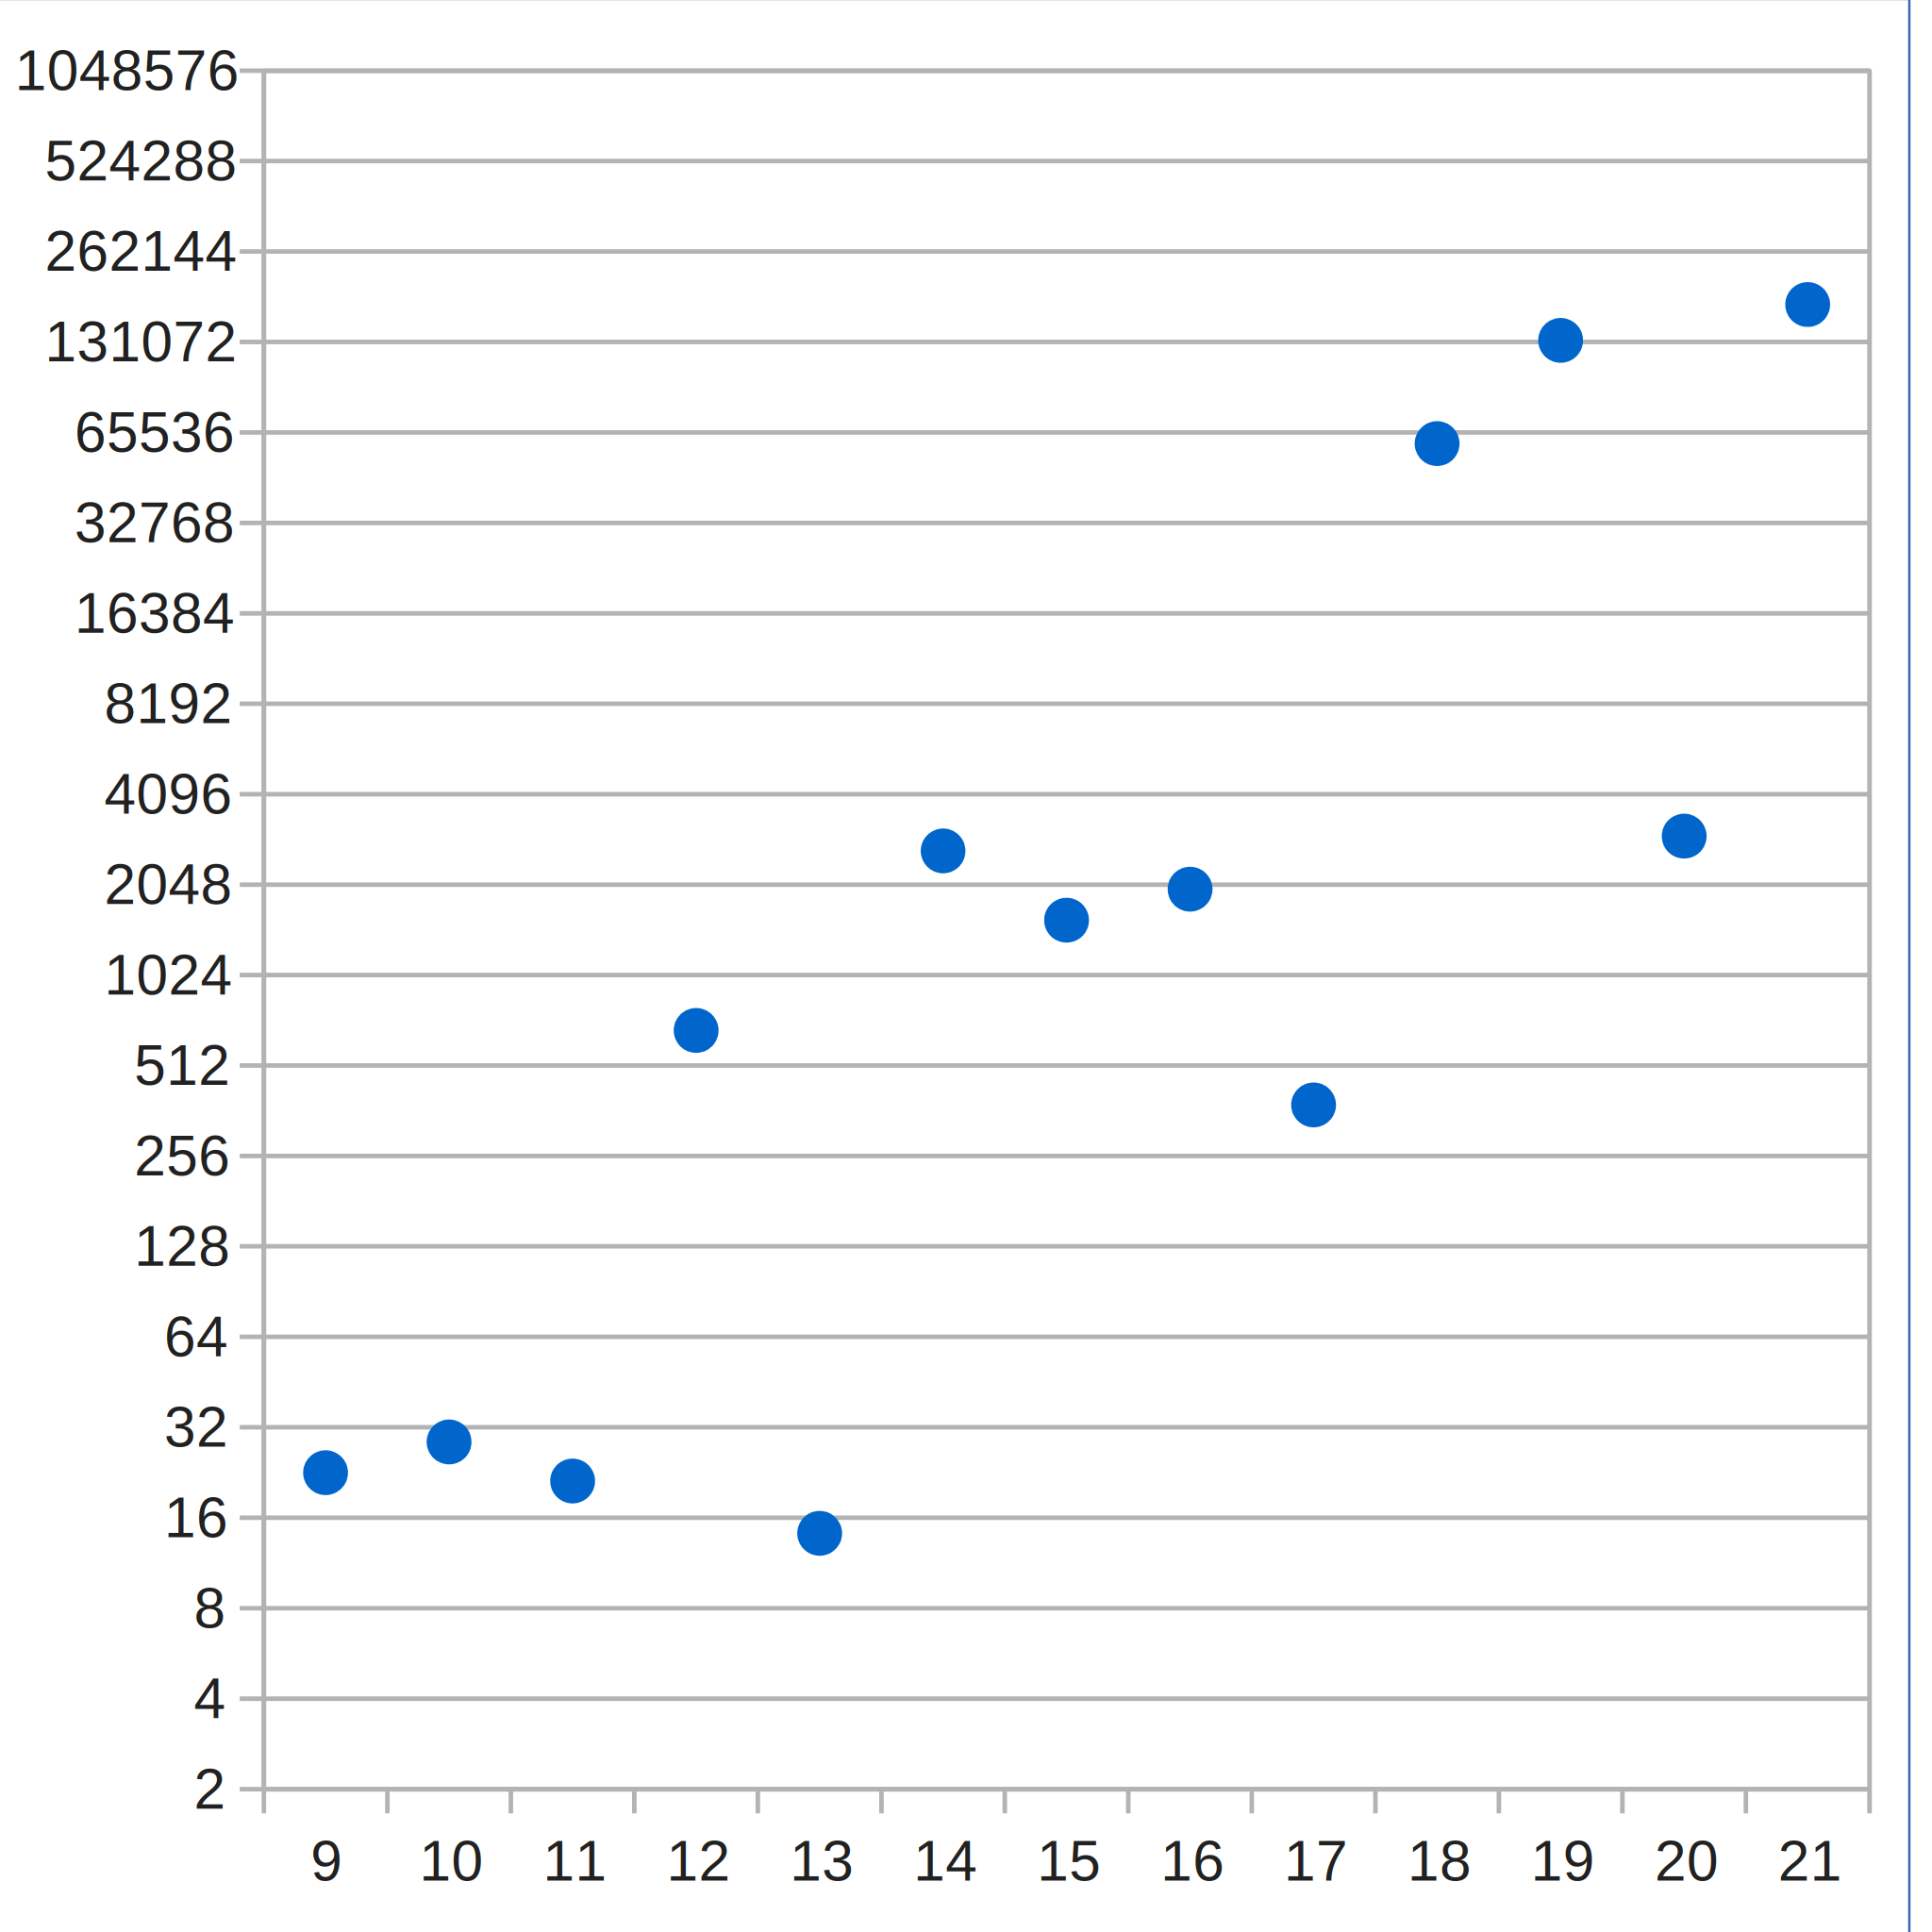
\includegraphics[scale=0.55]{images/eval_thesis}
  \end{minipage}
  \caption{Eigene Implementierung}
  \label{fig:eval_thesis}
\end{figure}

\begin{figure}[!h]
  \centering
  \begin{minipage}[t]{0.45\textwidth}
  \begin{flushleft}Gesamtdauer: TODO\end{flushleft}
  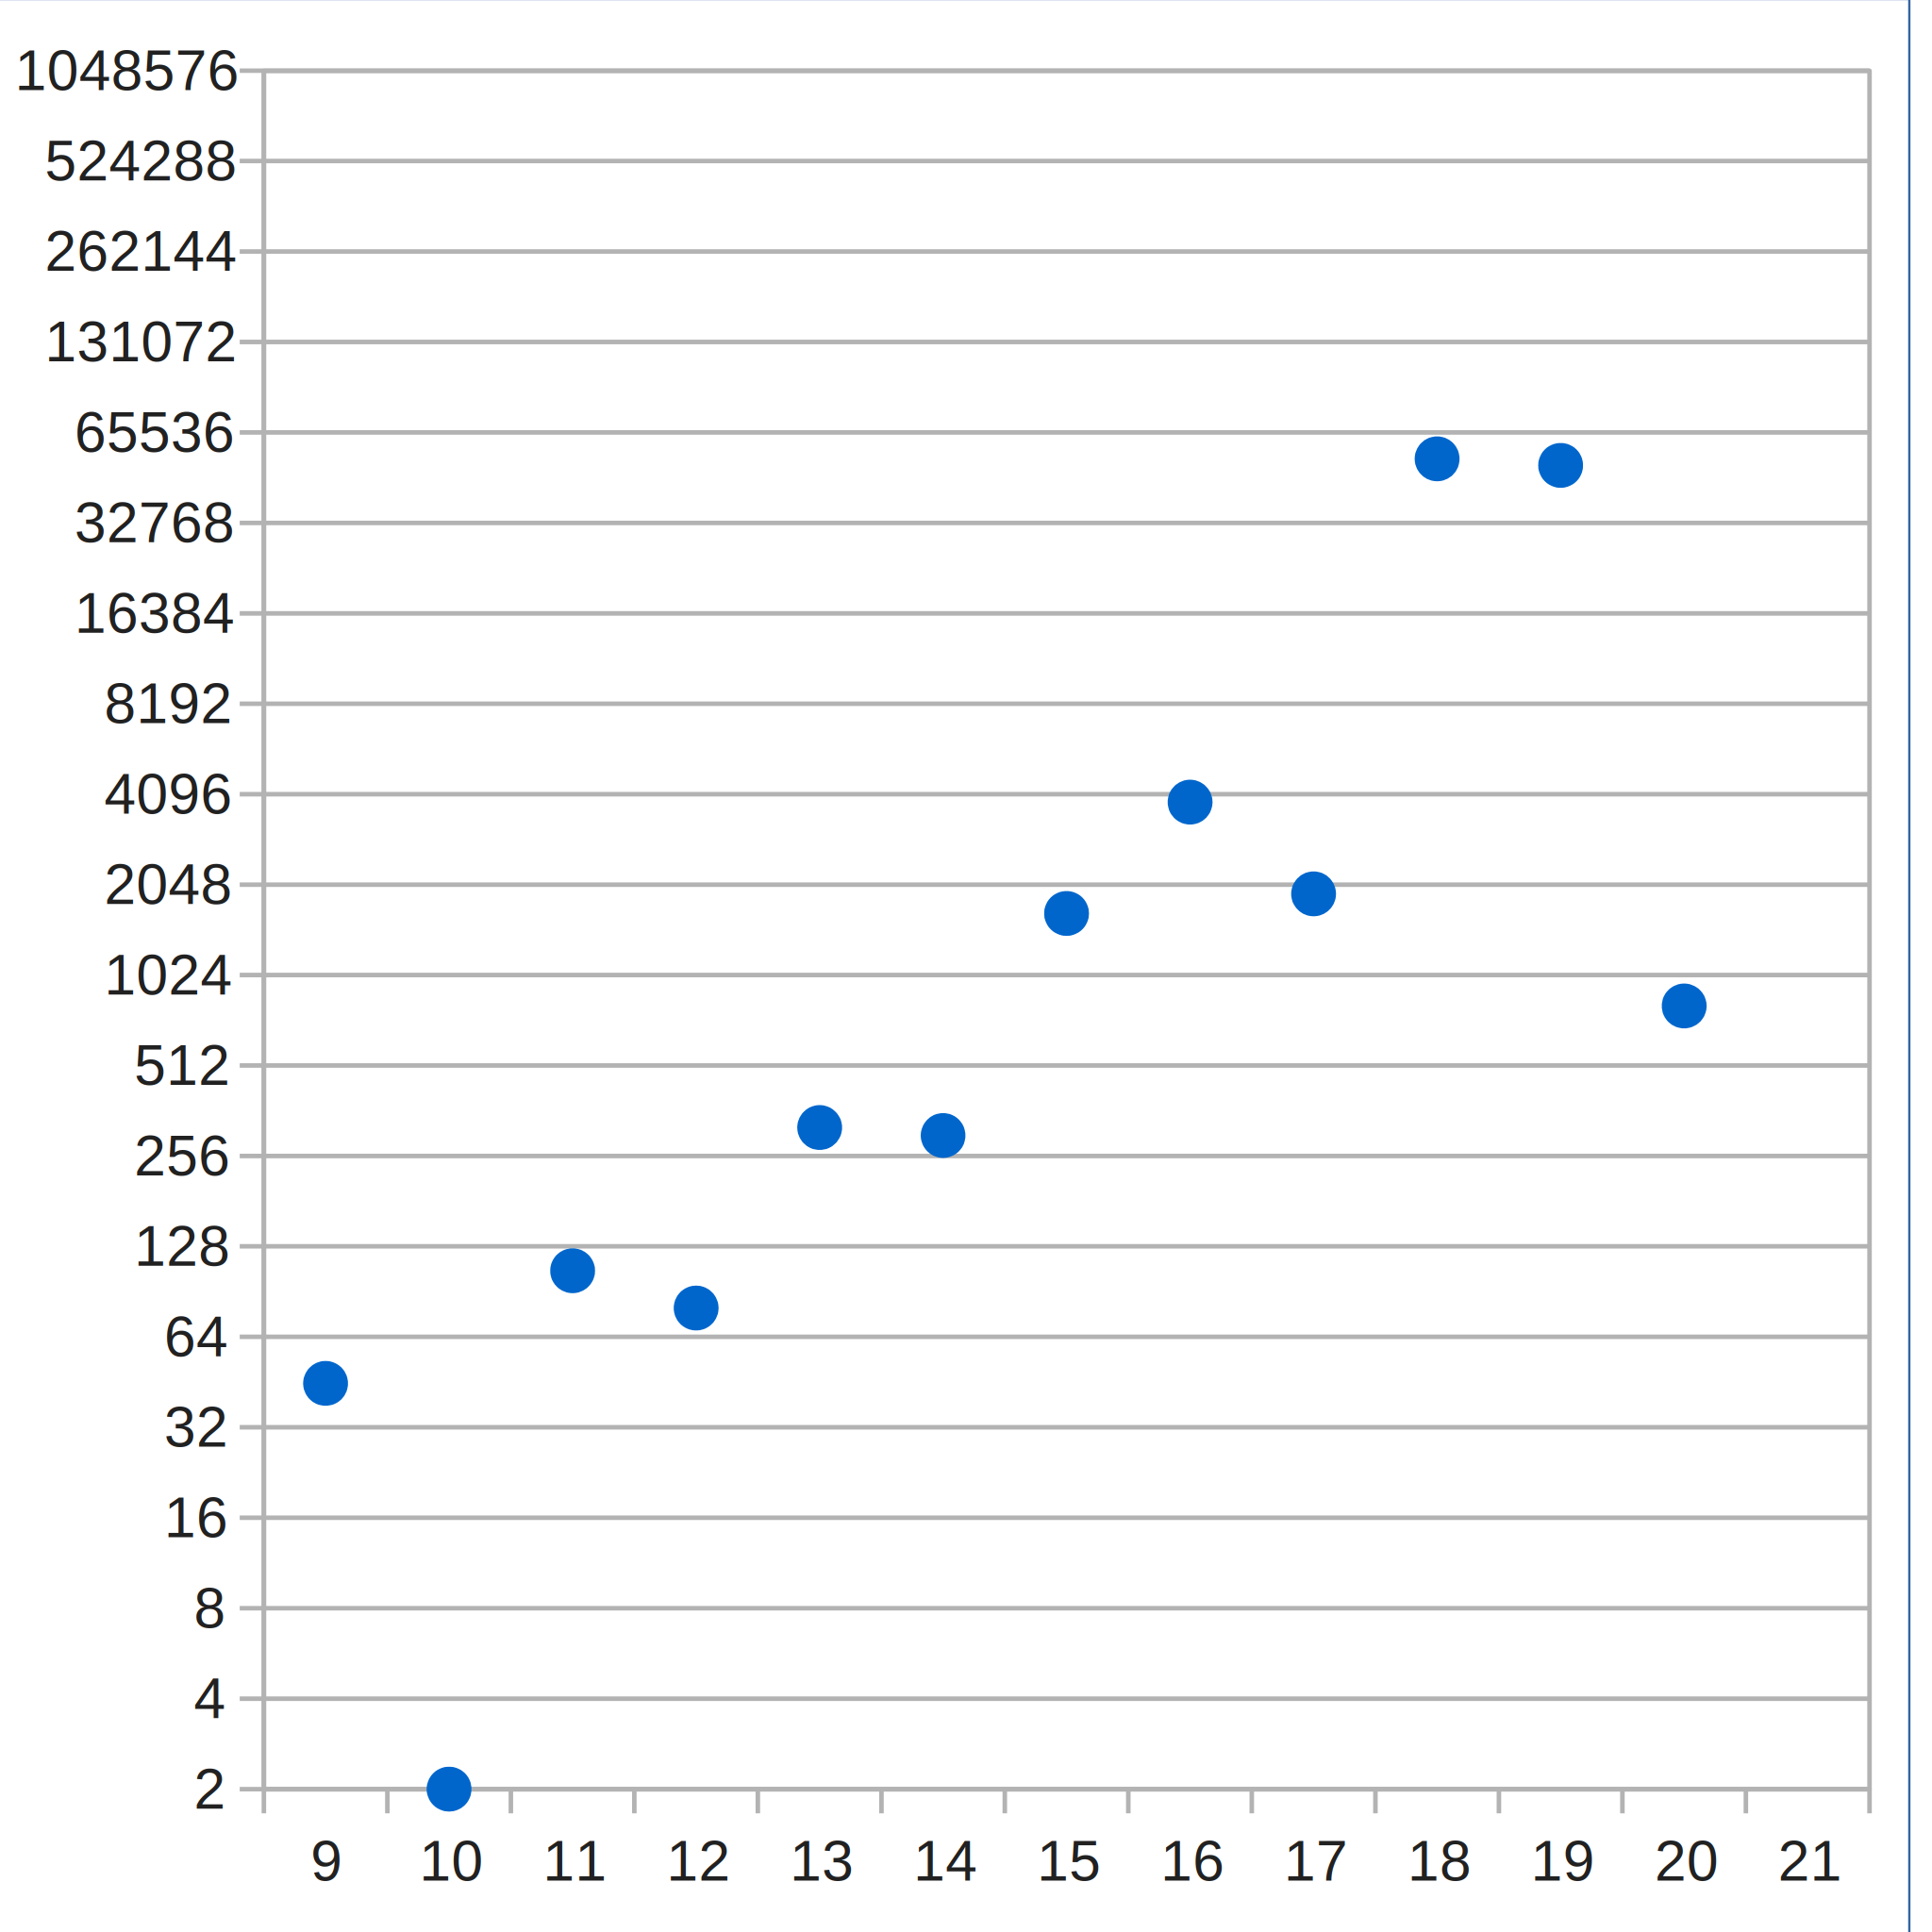
\includegraphics[scale=0.55]{images/eval_cbmc}
  \end{minipage}
  \caption{CBMC}
  \label{fig:eval_cbmc}
\end{figure}

\begin{figure}[!h]
  \centering
  \begin{minipage}[t]{0.45\textwidth}
  \begin{flushleft}Gesamtdauer: TODO\end{flushleft}
  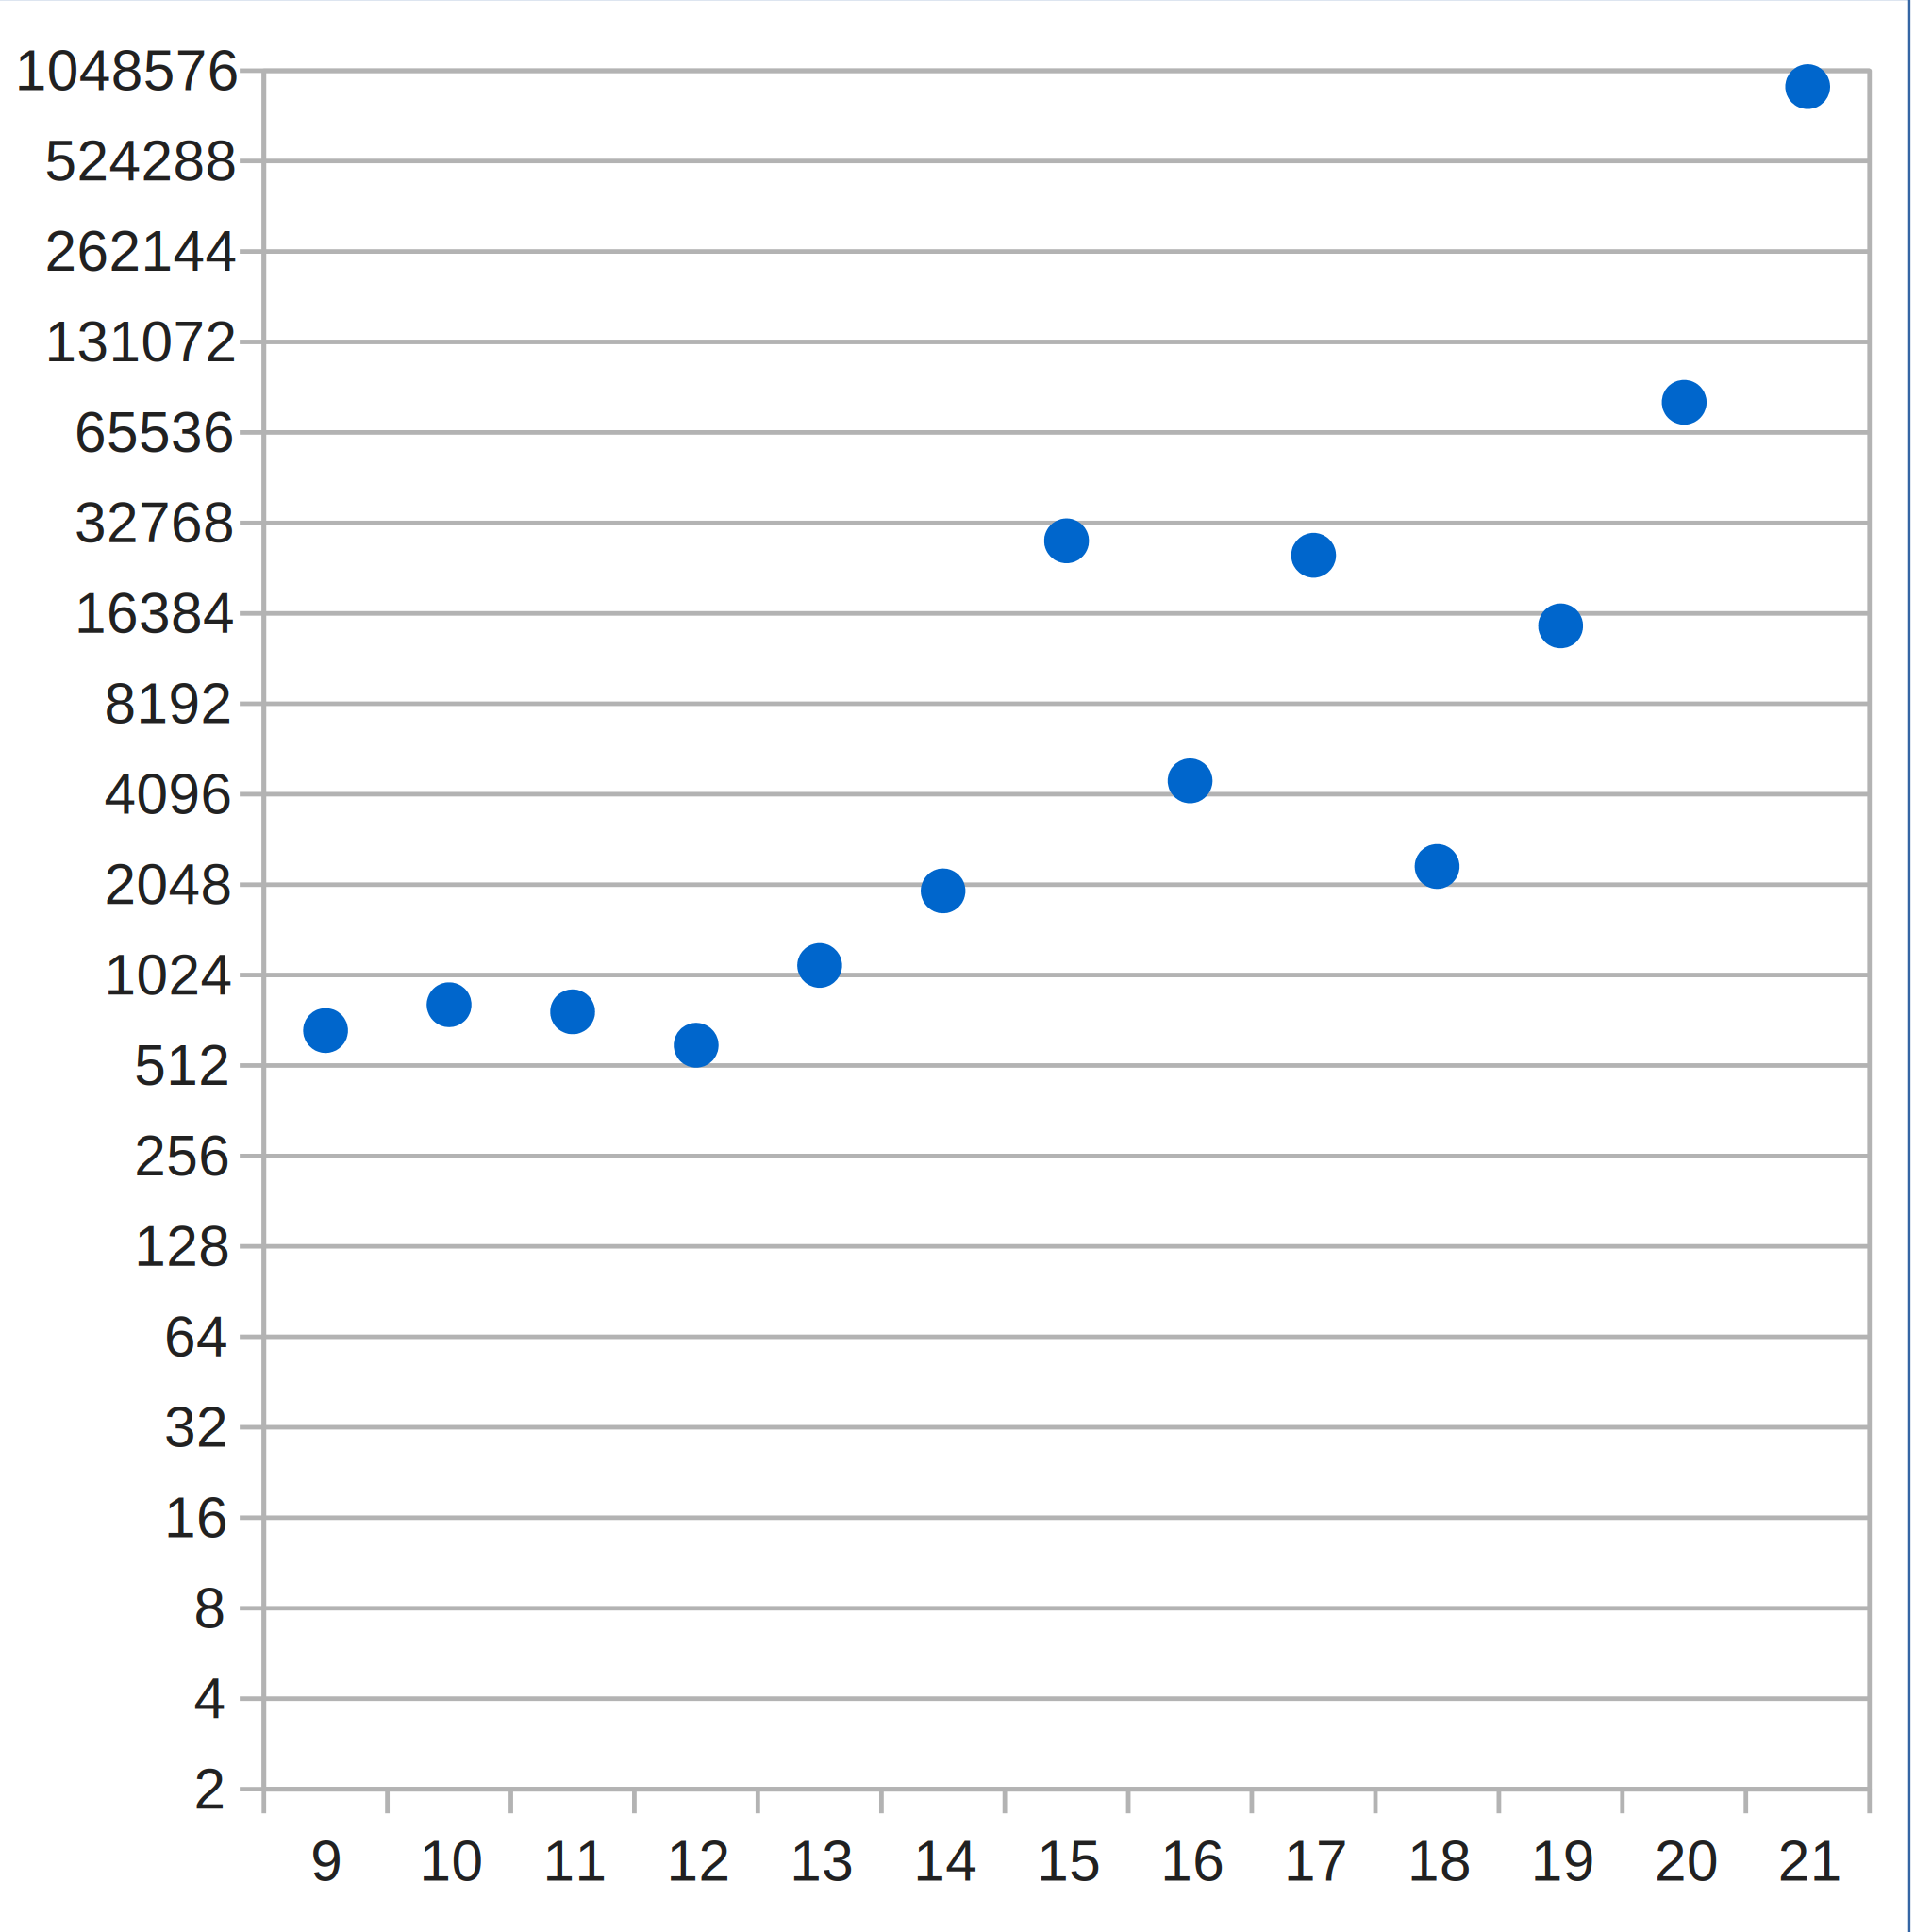
\includegraphics[scale=0.55]{images/eval_maurer-espresso}
  \begin{flushleft}Espresso\end{flushleft}
  \end{minipage}
  \begin{minipage}[t]{0.09\textwidth}
  ~~
  \end{minipage}
  \begin{minipage}[t]{0.45\textwidth}
  \begin{flushleft}Gesamtdauer: TODO\end{flushleft}
  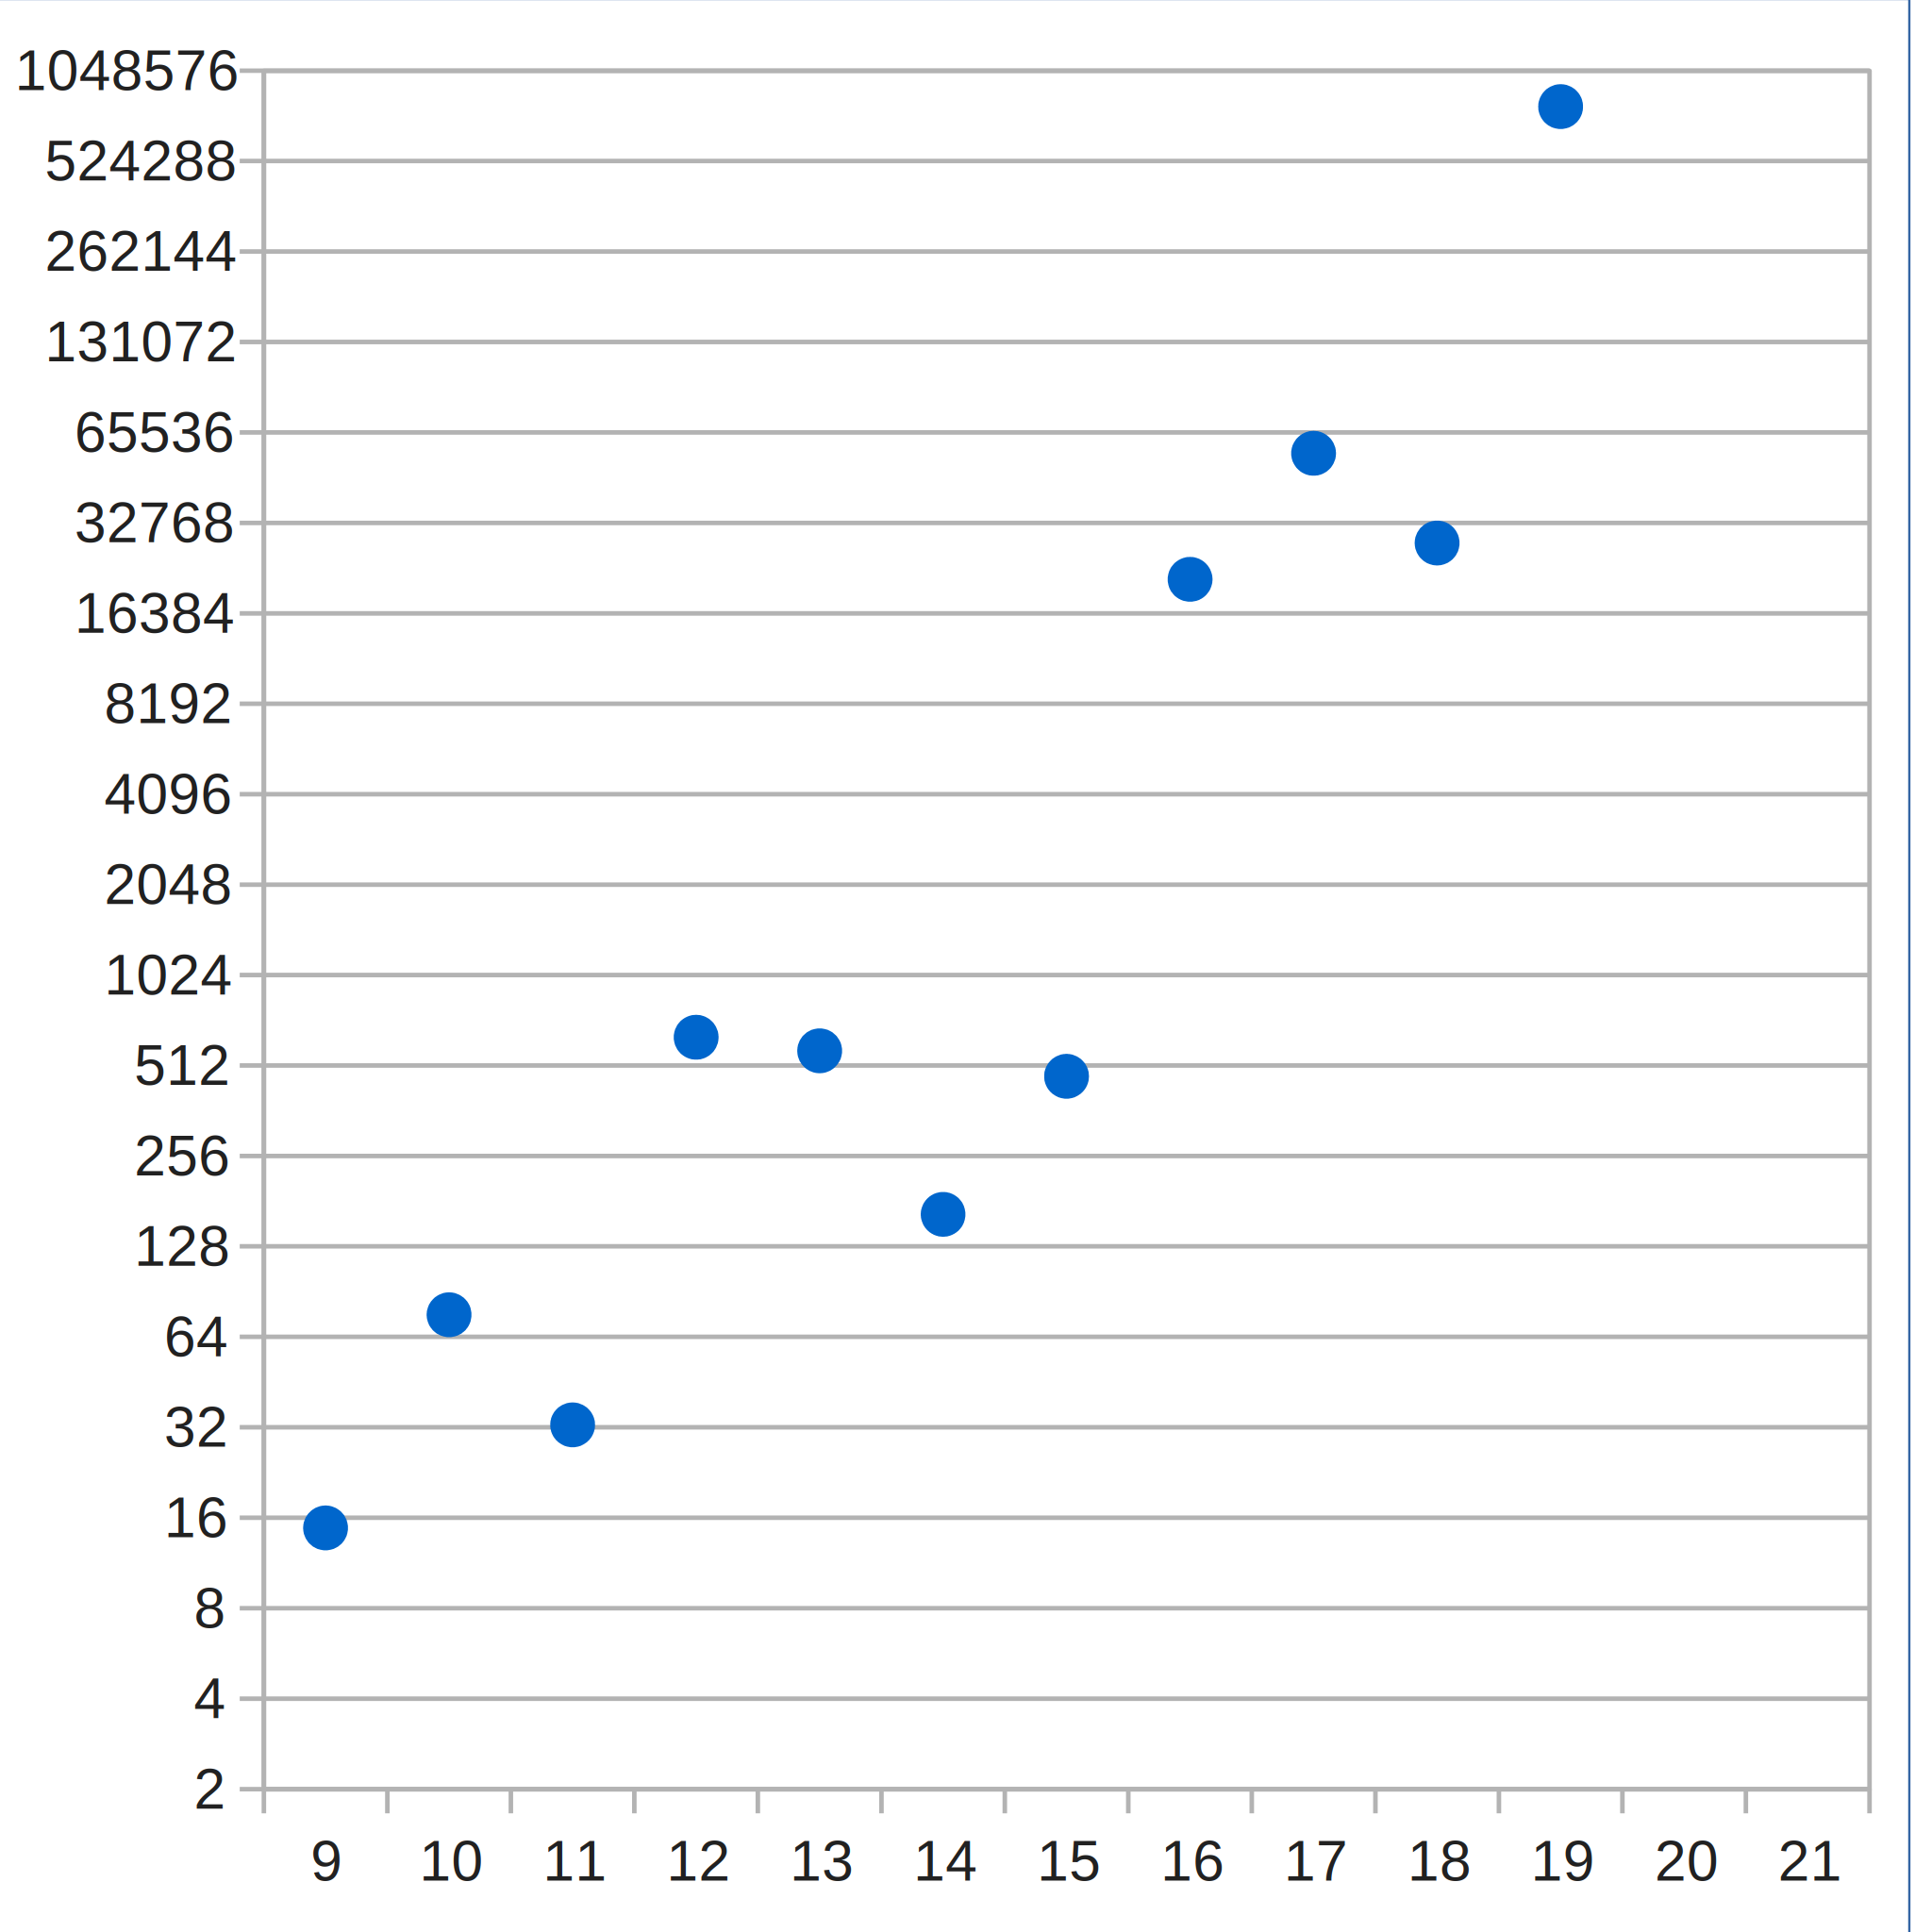
\includegraphics[scale=0.55]{images/eval_maurer-tseitin}
  \begin{flushleft}Tseitin\end{flushleft}
  \end{minipage}
  \caption{Martin Maurer}
  \label{fig:eval_maurer}
\end{figure}

\begin{figure}[!h]
  \centering
  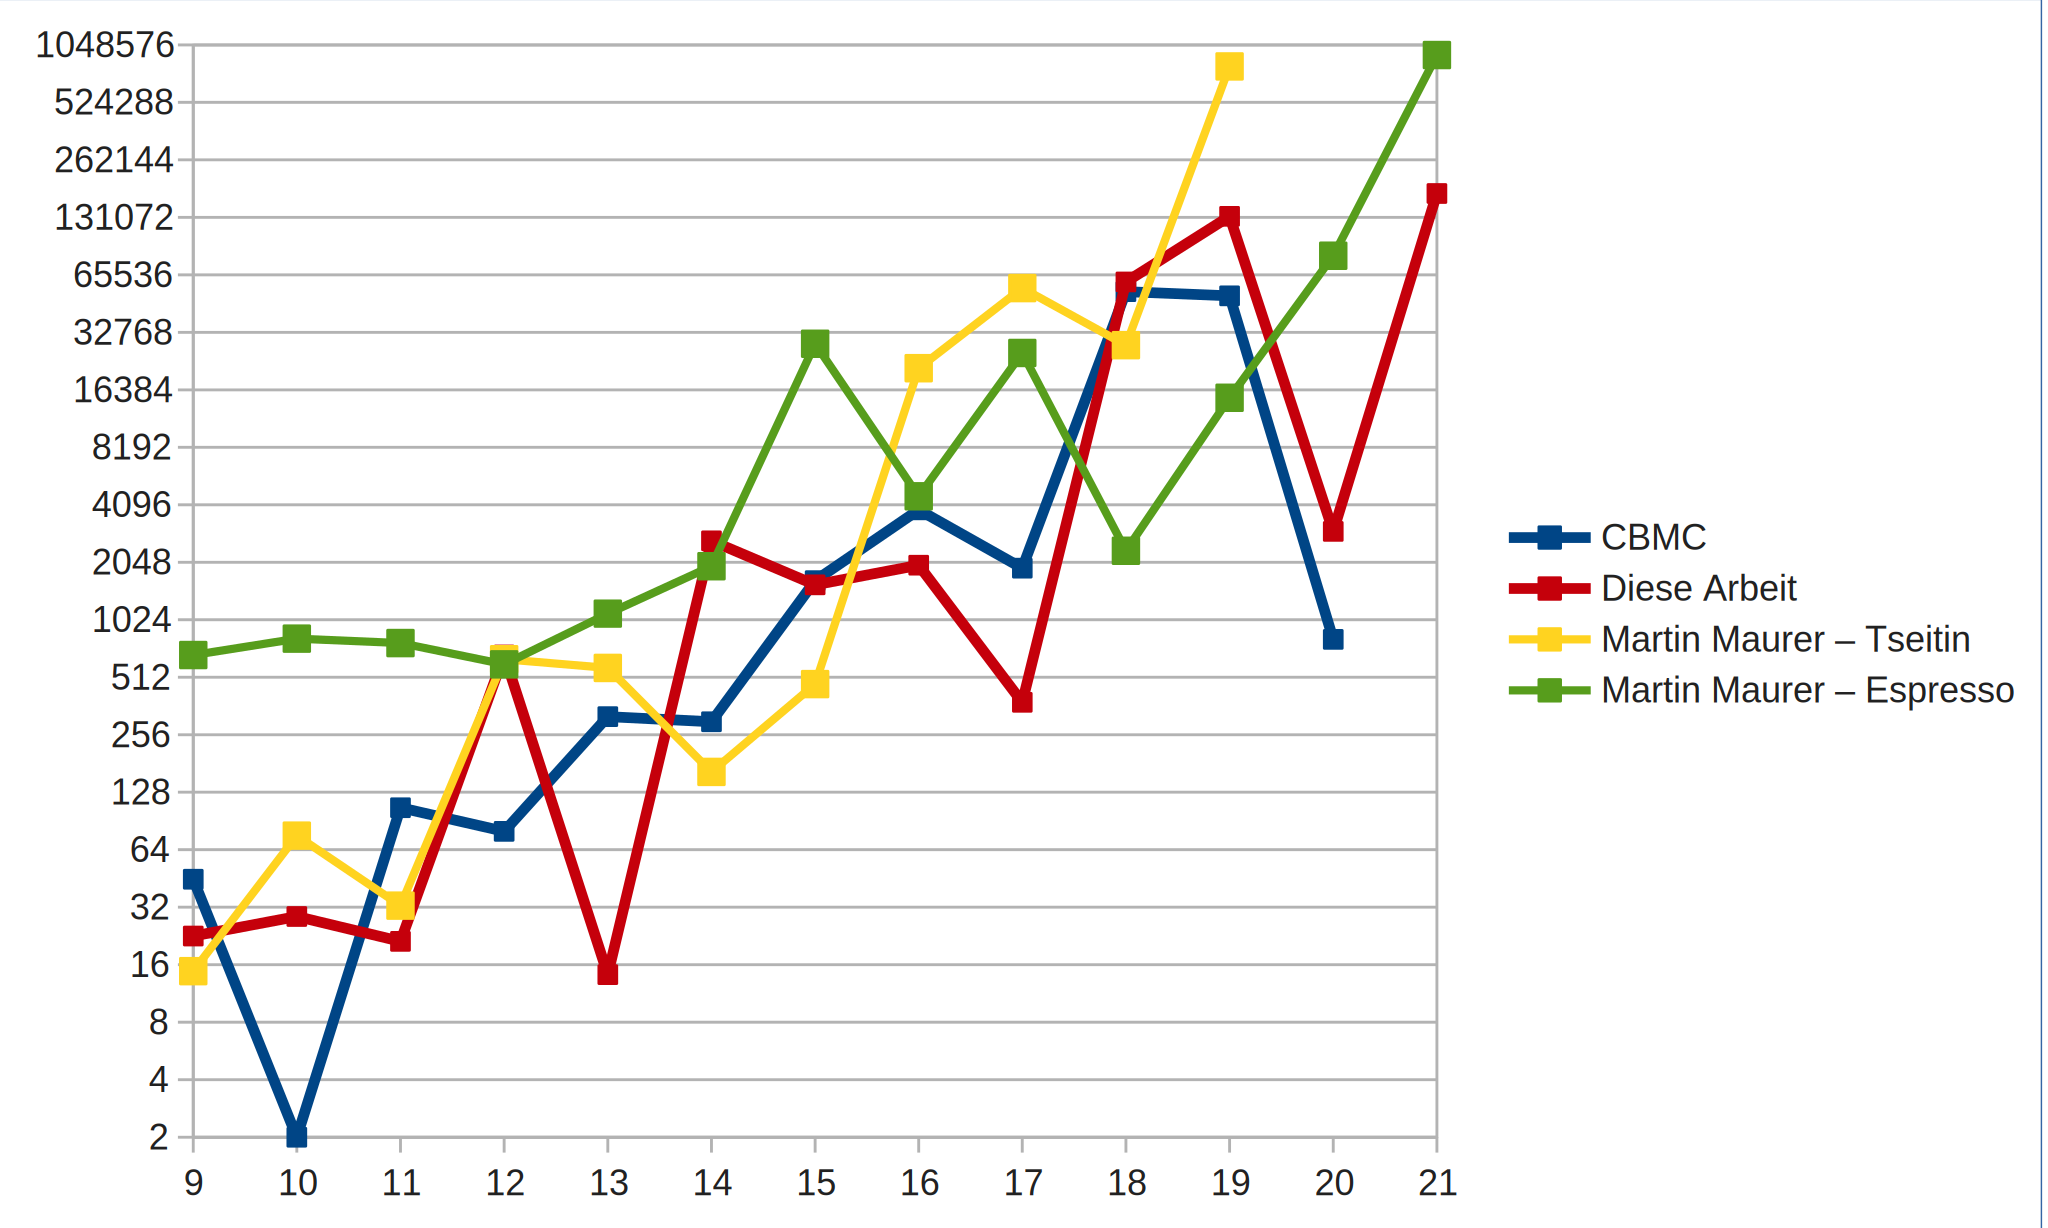
\includegraphics[scale=0.55]{images/eval_final}
  \caption{Eigene Implementierung}
  \label{fig:eval_final}
\end{figure}
\section{Bedeutung für SHA256}

\TODO{erledigen}

\subsection{Urbildberechnung}

\subsection{Initialwertberechnung}

\subsection{Kollisionsberechnung}
\section{Bitcoin-Mining}

\TODO{erledigen}